% Chapitre sur le rapport de recherche :


\chapter{Research report} 


\section{Problematic}


I mainly focused on membrane segmentation prior to arriving in the Megason lab. This is a challenging problem, as shown by the data analysis : the membrane data is incomplete, noisy, three dimensional and anisotropic.

Having no prior knowledge on Kishore's data denoising, I focused on level sets techniques to segment the membrane.
The level set theory provides a very flexible framework for segmentation problems. They are easily extensible to any dimension.
The drawbacks are that they are computationally intensive, and that the topology of the segmented region is by principle not controlled.

Similarly to region growing algorithms, level set algorithms can be initialized to provide prior information.
I focused on growing a levelset function from cells center. For that purpose, we need a good cell localization.
I have been studying levels sets in Creatis, for the purpose of cell segmentation and had some results in two dimensions.
I was then considering that nuclei were already correctly detected and segmented.
But when i arrived in the Megason Lab, I realized that before trying to segment the membrane using the techniques I studied in Creatis, I would need a correct cell nuclei detection.
We decided with Kishore that there was improvements to be brought to the cell nuclei detection algorithms.

That's why I started being interested in the problem of nuclei detection, in 3D confocal data.
After experiencing with Kishore's techniques, I implemented a recent algorithm for comparison, and proposed a new technique, with Dr Arnaud Gelas.


\chapter{My Proposals}

%
%\section*{Introduction}
%
%\subsection*{}
%
%\TODO{elle pue cette intro}
%I am presenting in this chapter, the research project I have been working on during the PFE. I have first undergone a bibliographic step, to acquire knowledge about the matter. Thanks to this research, I could determine which problems are still to be solved. Then I tried to find appropriate solutions to the problems encountered.
%
%The main difficulty in research, is that very often, there is no solution yet to the problem, in the domain. Therefore, I have had to do a bibliography, in order to determine the state of the art, and eventually learn some new theories.
%
%The image processing domain is particular: many algorithms are invented and published, but very few are available nor applicable to diverse images.
%Thus, there is a re-programming and evaluation step, prior to any innovation.

\subsection*{}

While in the Megason Lab, I have been working on segmenting fluorescent microscopy images.
Datas are four-dimensional (space and time), and represent regions (ear, brain...) of a developing zebrafish.
It is possible to visualy distinc nuclei and membranes of cells. Those elements constitute the basis of the model that we try to create.
Therefore, we have to be able to detect and track every cell across time. The model will also have to integrate morphological informations of each cell.

The creation of this model is a thesis subject : cells lineage registration in microscopy, during which I would like to extend my work.

Prior to arriving in the laboratory, I have been working on cell membrane. I have then concentrated my researches on cell nuclei detection and localization.




%
%  STATE OF THE ART
%

\section{State of the art in the megason lab}

\subsection{The Megason lab imaging pipeline}

Dr Kishore Mosaliganti has been working for two years in the Megason lab, in order to develop new segmentation methods for fluorescent images.
He has been working on experiencing and developing diverse algorithms for nuclei and membrane detection and segmentation.
As presented is the previous section, the datasets in the Megason Lab are extremely challenging:
they are huge and present important drawbacks (resolution, noise) as they are provided for visual processing and not computer assisted processing.

As these datasets are very big, and four dimensional, it is not possible to use Matlab for easy prototyping and experiencing : 
most of the time, the very low resolution third dimension will considerably modify the results.
There is also a time issue : the datasets must be treated in an acceptable amount of time,
and that prevents us from using Matlab language that does not provide every optimized function that we need for 3D images visualization and processing.
This forces us to program and prototype in {\C++}. The standard library used for image processing in the Megason Lab is ITK. Kishore's algorithm are all coded with this library.
The data processing in ITK is represented by pipelines : a series of connected filters that perform image processing tasks.
The Megason lab aslo develops a visualization program for microscopy data: {\gofigure}. This program uses ITK and VTK for processing and visualization of data. The long term goal being to include the algorithms to {\gofigure}, we also have to use those libraries.

Kishore studied several pipelines for nuclei and membrane segmentation.
For nuclei segmentation, an approach based on detection of nuclei, and region growing with the level set theory was used last year.
This year, a new approach based on nuclei detection and watershed algorithms is being used.
The algorithm used are standard and contour based for the detection of nuclei.
This leads to many errors in detection, due to the poor image quality. Right now, these errors are compensated after the segmentation step.

For membrane segmentation, Kishore is proposing a very good denoising technique based on anisotropic diffusion and tensor voting.
The reconstruction of the membrane structure is effective, even in low quality images. A segmentation step has to be implemented on top of it.


%
%  SEEDING
%

As chapter~\ref{} demonstrate, datas are hard to proceed. That forces us to find innovative solution for problems that may seem simple at first glance.

\section{Cell nuclei detection}

Cell nuclei shapes varies from spherical to curved ellipsoidal. As introduced above, the microscopy images are challenging, they are very noisy and anisotropic.
The main encountered difficulty is clustered nuclei that result from the point spread function of the microscope and the low resolution in the third dimension.

The algorithms used in the Megason lab for nuclei and membrane segmentation are based on an initialisation inside the nuclei.
Right now, a composite algorithm is used for detecting these nuclei based on a combination of contour based algorithms (see~\ref{sect:megasonExisting}).
This method gives good enough results for starting a watershed algorithm. Segmented regions that obviously don't correspond to a cell nucleus are eliminated. The final result of the segmentation process is evaluated.
\TODO{cite Kishore papers}


This is clear that  the nuclei detection has to be improved.
I started by carying a bibliographic research, to determine the state of the art in the nuclei segmentation/detection domain.
Then, I implemented a new algorithm based on the Laplacian of Gaussian method.
After that, I created an evaluation framework, to compare the results given by this new algorithm, and Kishore's.
We finally proposed a new method taking advantage of the cell membrane information.



\subsection{Existing methods}

There are several papers dealing with cell nuclei or cell detection 
\cite{loukas2003image,umesh2001efficient,al2009improved},
but only one is based on 3D confocal images~\cite{li20073}, similar to the ones acquired in the Megason lab.

\subsubsection*{Confocal nuclei detection}
G. Li {\etal}~\cite{li20073}, describe a segmentation method for nuclei in 3D confocal datasets. The method they use is based on gradient vector flow tracking.
The image processing pipeline is presented figure~\ref{fig:gradientflowFlowchart}.
\begin{description}
  \item[Data] are 3D confocal datasets from zebrafish embryos. They are fluorescent nuclei.
  \item[Method] is described figure~\ref{fig:gradientflowFlowchart}. 
  A re-sampling and spline based interpolation is performed on the original data to get isotropic datasets.
  The gradient vector diffusion field (see figure~\ref{fig:gradientflowFlowfield}) is then computed on a Gaussian blurred version of the isotropic data.
  Following \cite{bajcsy1989multiresolution}, an elastic constraint is added to the diffusion equation to get a smooth vector field.
  The tracking consists in selecting some points and moving them according to the vector field. The resulting trajectories end in "sinks" that correspond to center of nuclei.
  A refinement step groups the close "sinks".
  The segmentation is the done by cropping the image around each nuclei and applying a local adaptive threshold to find one nuclei per subregion.
  A final step consists in eliminating the false positives (nuclei which are too small).
  \item[Evaluation] is performed on 10 confocal datasets. The mean amount of nuclei in the datasets is 310. The number of over segmented and under segmented nuclei is presented. The automatic segmentation result is compared with the segmentation of two experts.
  \item[Results] the algorithm provides good results in the paper: 
  4.93\% of over-segmented nuclei,
  and 5.03\% of under-segmented nuclei.
  \item[Comments]:
  The article misses the part describing the region cropping for getting the regions where the adaptive
   threshold should be computed.
   Looking at the illustration, it seems like these regions are either determined
   according to attraction basins of each sink, or with a constrained Voronoi diagram.
\end{description}
\begin{figure}[h]
\begin{center}
\leavevmode
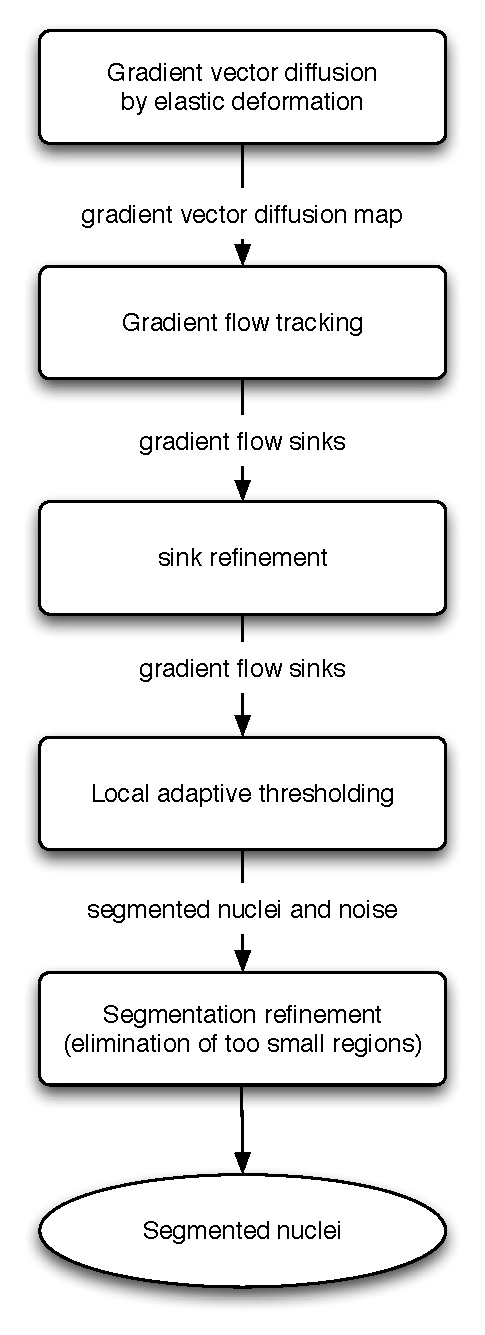
\includegraphics[height=0.75\textheight]{pictures/gradientflowFlowchart}
\end{center}
\caption{Flowchart of the algorithm proposed in~\cite{li20073}}
\label{fig:gradientflowFlowchart}
\end{figure}

\begin{figure}[h]
  \centering
  \captionsetup[subfloat]{labelformat=empty}
  \subfloat[][]{{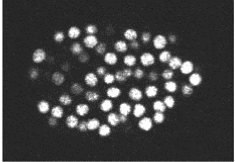
\includegraphics[width=0.33\textwidth]{pictures/gradientflowSegmenta}\label{fig:gradientflowSegmenta}}}
  \subfloat[][]{{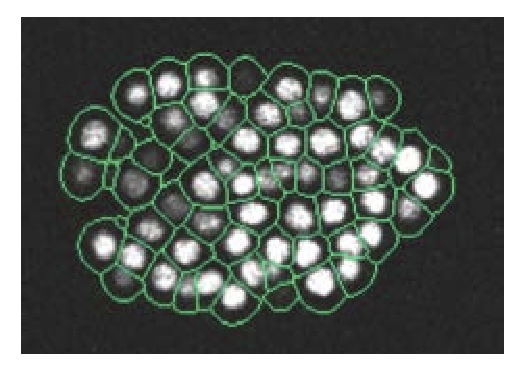
\includegraphics[width=0.33\textwidth]{pictures/gradientflowSegmentb}\label{fig:gradientflowSegmentb}}}\\
  \subfloat[][]{{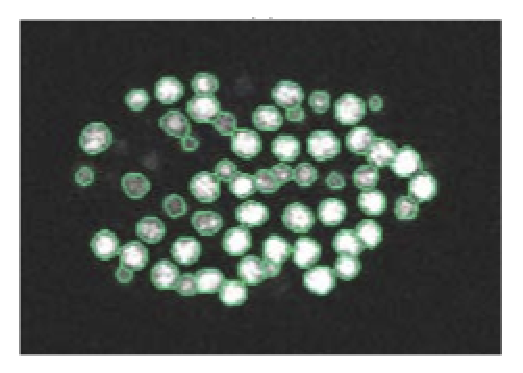
\includegraphics[width=0.33\textwidth]{pictures/gradientflowSegmentc}\label{fig:gradientflowSegmentc}}}
  \subfloat[][]{{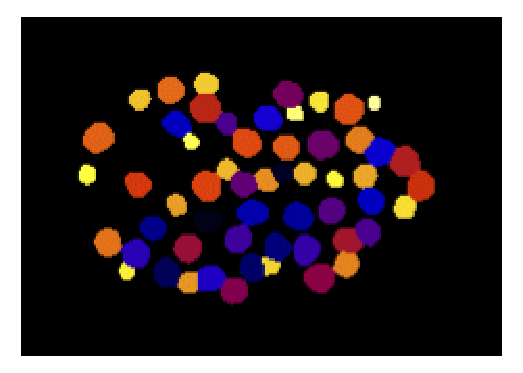
\includegraphics[width=0.33\textwidth]{pictures/gradientflowSegmentd}\label{fig:gradientflowSegmentd}}}
\caption{%
Illustration of 3D cell nuclei segmentation on a 2D slice, from~\cite{li20073}.
\subref{fig:gradientflowSegmenta}: A slice from 3D cell nuclei image;
\subref{fig:gradientflowSegmentb}: Boundaries of small regions overlaid on the slice;
\subref{fig:gradientflowSegmentc}: Edges of cell nuclei overlaid on the slice after the step of adaptive thresholding;
\subref{fig:gradientflowSegmentd}: Randomly color-coded extracted cells.}
\end{figure}

\begin{figure}[h]
  \centering
  \captionsetup[subfloat]{labelformat=empty}
  \subfloat[][]{{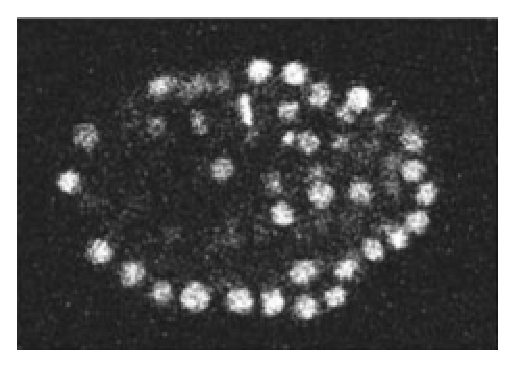
\includegraphics[width=0.5\textwidth]{pictures/gradientflowFlowfielda}\label{fig:gradientflowFlowfielda}}}\\
  \subfloat[][]{{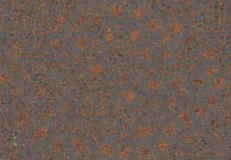
\includegraphics[width=0.33\textwidth]{pictures/gradientflowFlowfieldb}\label{fig:gradientflowFlowfieldb}}}
  \subfloat[][]{{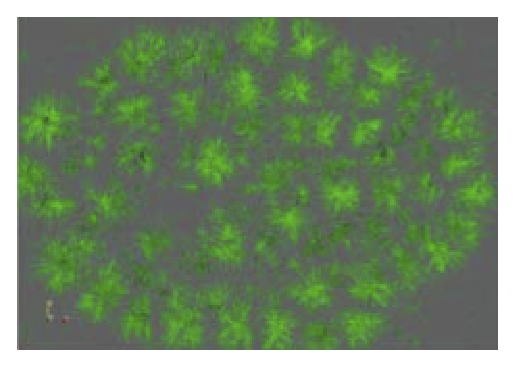
\includegraphics[width=0.33\textwidth]{pictures/gradientflowFlowfieldc}\label{fig:gradientflowFlowfieldc}}}\\
  \subfloat[][]{{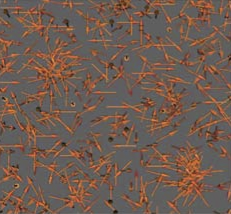
\includegraphics[width=0.33\textwidth]{pictures/gradientflowFlowfieldd}\label{fig:gradientflowFlowfieldd}}}
  \subfloat[][]{{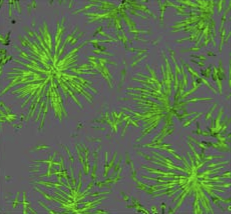
\includegraphics[width=0.33\textwidth]{pictures/gradientflowFlowfielde}\label{fig:gradientflowFlowfielde}}}
\caption{%
The 3D view of gradient vector field and diffused gradient vector field with elastic deformation transformation of a slice cropped from a 3D cell nuclei image, from~\cite{li20073}.
\subref{fig:gradientflowFlowfielda}: A slice of the 3D image;
\subref{fig:gradientflowFlowfieldb}: The original gradient vector field;
\subref{fig:gradientflowFlowfieldc}: The diffused gradient flow field with elastic deformation transformation;
\subref{fig:gradientflowFlowfieldd}: Zoomed view of \subref{fig:gradientflowFlowfieldb};
\subref{fig:gradientflowFlowfielde}: Zoomed view of \subref{fig:gradientflowFlowfieldc}.}
\end{figure}
\clearpage

\subsubsection*{3D histological pathological cell detection}
 P.S. Umesh Adiga {\etal}~\cite{umesh2001efficient}, present a method for segmenting cells in histological images 
  (which are somehow close to nuclei in fluorescent images).
  \begin{description}
  \item[Data] are 3D confocal histo-pathological images of cells in thick tissues.
  \item[Method] is described figure~\ref{fig:watershedFlowchart}.
  A first step consists in thresholding the image to keep only the nuclei. The threshold level is given by an empirical law based on the histogram of the images.
  Then, a succession of mathematical morphology operations consisting in opening and closing with a structuring element of same size, are used to improve the data. 
  This filters the texture of the cells, and removes holes.
  An intensity correction is then applied along the z axis. The figure~\ref{fig:watershedPrefilt} illustrates the results of this pre-processing.
  After a binarization of the preprocessed image, a distance map is computed and thresholded to find the cell markers, to initiate the watershed algorithm.
  Once the watershed algorithm has converged, a region merging process groups over-segmented cells. The region merge used in this paper is described by figure~\ref{watershedMerge}.
  \item[Evaluation] is performed on 15 3D datasets. The mean amount of nuclei in the datasets is 22. The information provided by the evaluation is the number of detected cells compared to the number of real cells present. No information is given on the type of error. The algorithm is compared to \cite{malpica1997applying}, and shows better performance according to the evaluation criterion.
  \item[Results] the algorithm provides very good results in the paper with 2\% of error instead of 9\% for \cite{malpica1997applying}.
  \item[Comments]: this article is well presented with a description of all the steps of the processing pipeline.
  The evaluation is done on small datasets (256*256*24) with few cells. A good information would have been amount of under segmented cells. 
\end{description}
\begin{figure}[h]
\begin{center}
\leavevmode
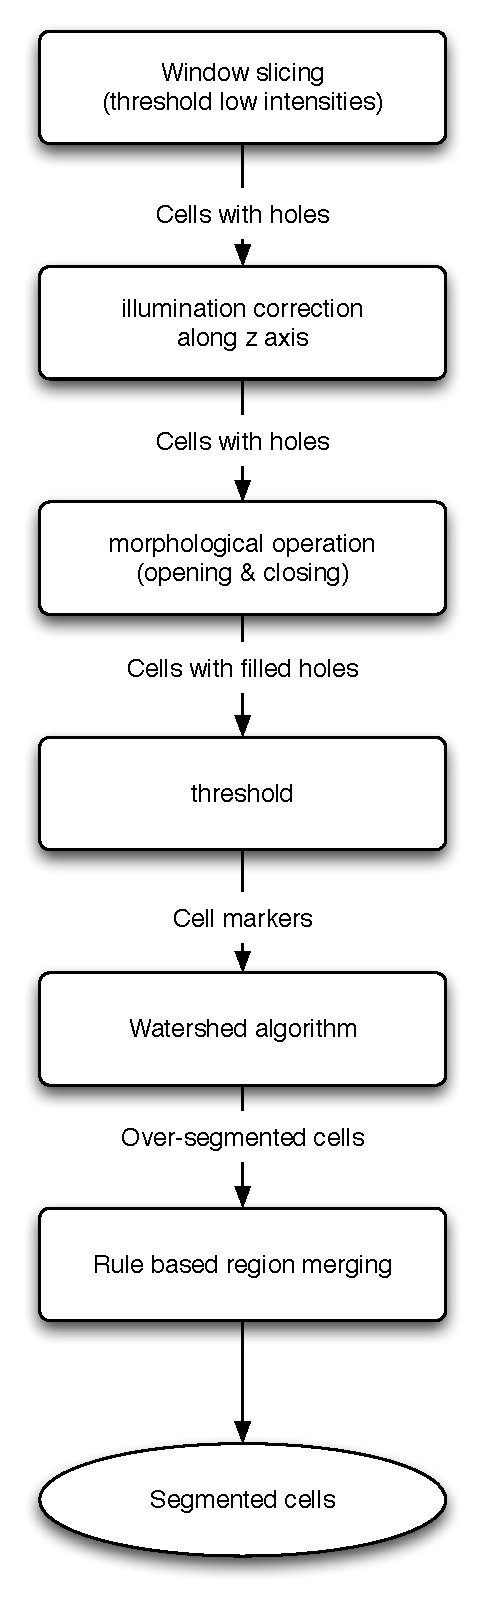
\includegraphics[height=0.75\textheight]{pictures/watershedFlowchart}
\end{center}
\caption{Flowchart of the algorithm proposed in~\cite{umesh2001efficient}}
\label{fig:watershedFlowchart}
\end{figure}
\begin{figure}[h]
  \centering
  \captionsetup[subfloat]{labelformat=empty}
  \subfloat[Diagrammatic representation of detecting the small fragments of the object and finding its parent.]{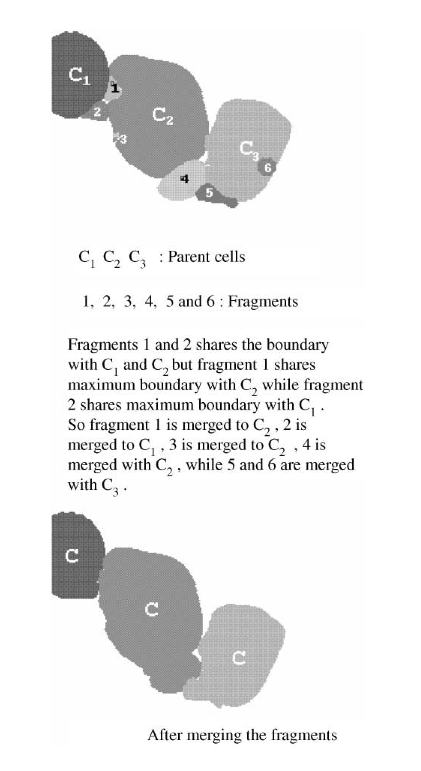
\includegraphics[width=0.49\textwidth]{pictures/watershedMerge}\label{fig:watershedMerge}}
\subfloat[Result of image enhancement steps shown over a single image slice: (a) original image slice, (b) result of window slicing, (c) result of size-filtering, (d) result of morphological opening and closing of a 3D image.]{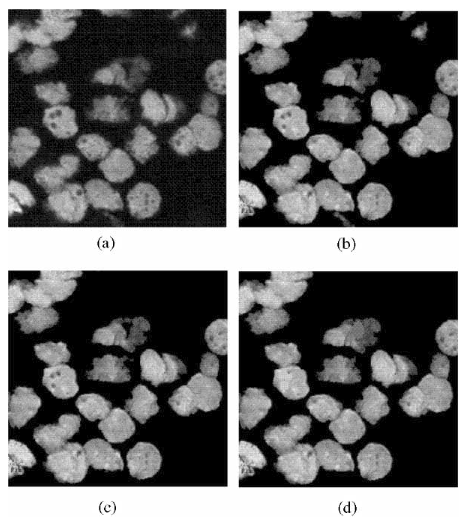
\includegraphics[width=0.49\textwidth]{pictures/watershedPrefilt}\label{fig:watershedPrefilt}}
\caption{illustrations from \cite{umesh2001efficient}}
  \label{fig:watershedIllustration}
\end{figure}
\clearpage


\subsubsection*{Histological cell nuclei detection}
\label{sect:farsight}
Yousef Al-Kofahi {\etal}~\cite{al2009improved}, presents a new method for nuclei detection.
  \begin{description}
  \item[Data] are 2D histological images (see figure~\ref{fig:farsightInitial}).
  \item[Method] is described figure~\ref{fig:farsightFlowchart}.
  A first step consists in finding the foreground of the image with a graph cut based binarization (illustrated figure~\ref{farsightBinary}).
  A distance map is then computed on this binary image, and is used to constrain the scales of a multiscale Laplacian of Gaussian (see~\ref{sect:MLOG}).
  The original image is processed by the scale-constrained multi-scale Laplacien of Gaussian.
  A local maxima detection is performed on the resulting scalar field (as shown figure~\ref{fig:farsightMLOG}).
  Those local maximas correspond to the position of the cell.
  A watershed algorithm is then initiated from these points, and finally refined by manual editing and "alpha-refinement".
  \item[Evaluation] is done on 25 images containing an average of 298 cells per image. The results present the number of over and under segmented cell nuclei and separates encroachment errors.
  \item[Results] the algorithm provides acceptable results : 13.7\% of error.
  \item[Comments]: this article is well presented with a description of all the steps of the processing pipeline.
  The evaluation is done on enough images, and the results are detailed.
  The algorithm was implemented in the Farsight toolkit (FTK, \url{http://www.farsight-toolkit.org/}), but we were unable to make it run on 3D data.
\end{description}
\begin{figure}[h]
\begin{center}
\leavevmode
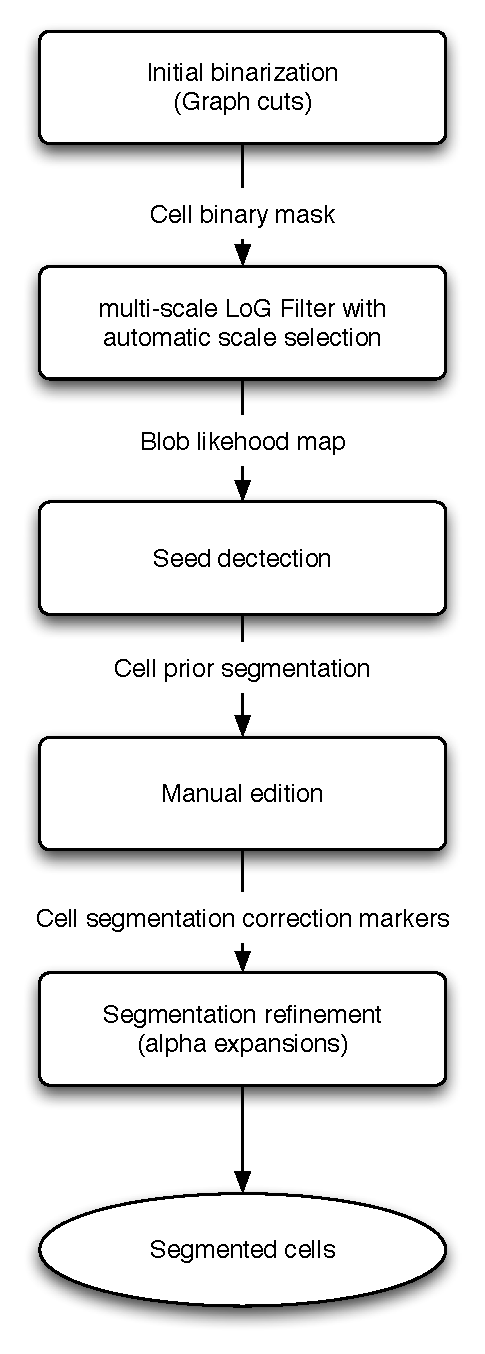
\includegraphics[height=0.75\textheight]{pictures/farsightFlowchart}
\end{center}
\caption{Flowchart of the algorithm proposed in~\cite{al2009improved}}
\label{fig:farsightFlowchart}
\end{figure}
\begin{figure}[h]
  \centering
  \captionsetup[subfloat]{labelformat=empty}
\subfloat[(A) Nuclear channel from spectral unmixing.]{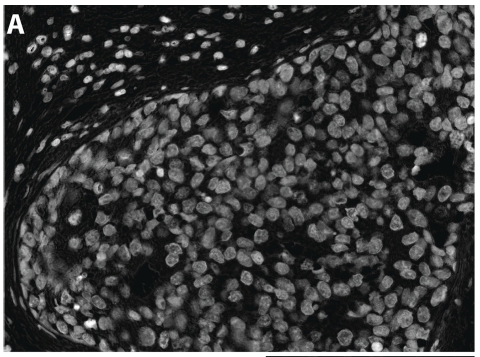
\includegraphics[width=0.49\textwidth]{pictures/farsightInitial}\label{fig:farsightInitial}}
\subfloat[(B) Foreground extraction results. Pixels marked yellow represent a large connected component.]{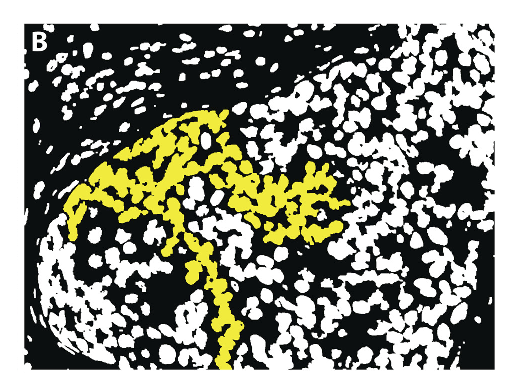
\includegraphics[width=0.49\textwidth]{pictures/farsightBinary}\label{farsightBinary}} \\
\subfloat[(C) Surface plot of the multiscale LoG filtering results for a small region. (D) Initial segmentation based on the LoG. (E) Surface plot of the distance-map-constrained multiscale LoG. (F) Improved initial segmentation resulting from the distance-constrained LoG.]{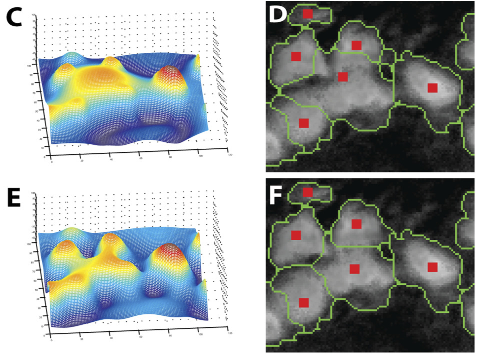
\includegraphics[width=0.75\textwidth]{pictures/farsightMLOG}\label{fig:farsightMLOG}}
\caption{illustrations from \cite{al2009improved}}
  \label{fig:farsightIllustration}
\end{figure}
\clearpage


\subsubsection{Existing method in the Megason Lab}
\label{sect:megasonExisting}
The existing method in the Megason Lab, for nuclei detection and segmentation, is also based on a detection of nuclei, and then, a segmentation, using watershed.
  \begin{description}
  \item[Data] are the challenging 3D confocal/2-photons images presented in the Data analysis part. 
  \item[Method] is described figure~\ref{fig:kishoreFlowchart},
  A pre processing stage consists in denoising the raw image, with an anisotropic diffusion filter.
  Then, the algorithm consists in a combination of methods : 
  hough transform, image masking and distance map, and the redial voting technique described in \cite{chang2007segmentation}, applied to the denoised image.
  Once the three filters processed the nuclei image, their output scalar fields are summed.
  A local maxima extraction is performed on this resulting field.
  This extraction filters the close local maximas, to reduce the noise impact, by selecting the highest local maxima, and ignoring the other local maximas in a certain radius.
  those maximas are then used for initializing a watershed algorithm.
  \item[Evaluation] has been visually carried out by Kishore, for the initialization points of the watershed.
  For the result of the watershed, the evaluation was performed on an expert-segmented dataset of 180 cell nuclei.
  \item[Results] are still to be evaluated.
  \item[Comments]: there is an existing method in the Megason lab, but it has not yet been evaluated nor published. Improving this method consists in, first going through the algorithms' code, then create a visualization and evaluation framework, and finally compare it with other methods.
\end{description}
\begin{figure}[h]
\begin{center}
\leavevmode
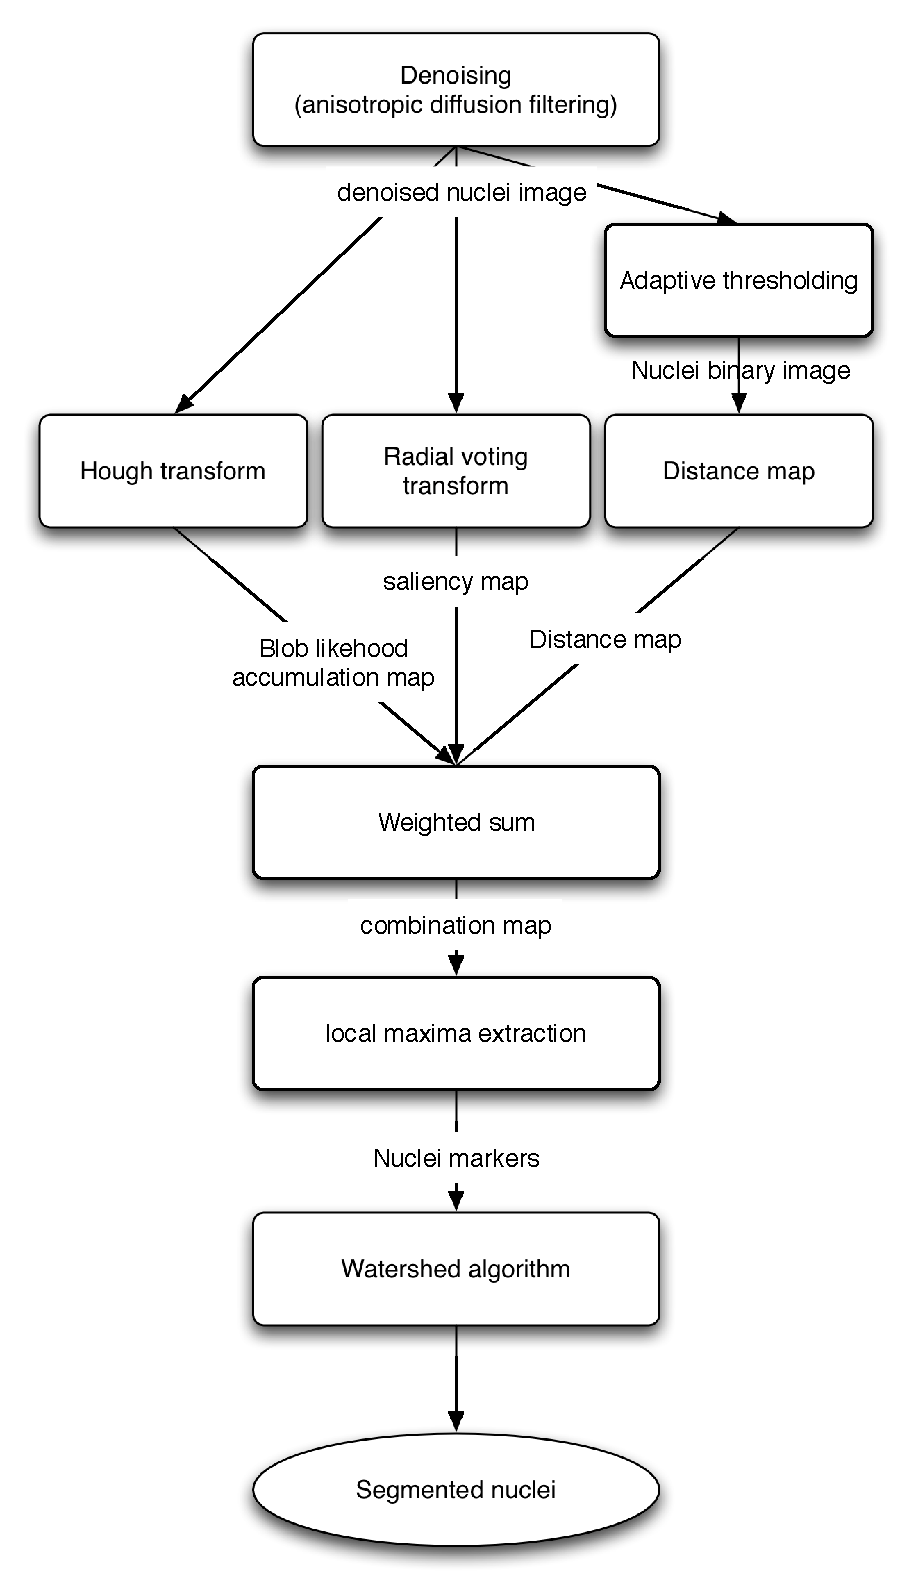
\includegraphics[height=0.75\textheight]{pictures/kishoreFlowchart}
\end{center}
\caption{Flowchart of the algorithm used in the Megason Lab}
\label{fig:kishoreFlowchart}
\end{figure}
\clearpage


\subsubsection*{Conclusion}

We can conclude that there are some existing algorithms for detecting and segmenting cell nuclei,
but very few were designed for 3D confocal data.
Most of the time, they perform well on 2D datasets, but are tricked by the low resolution of the third dimension.
The evaluation is most of times based on the final segmentation, and interesting informations are number of over/under-segmented cell nuclei.






\section*{Conclusion}


%A Context of the internship
%1- Biological Context / Goals
%2- Image Processing Challenges
%3- Data presentation
%4- The problem: you are going to address " ??? "
%
%B- Cell nuclei detection
%Intro
%1- State of the art
%2- What's wrong with existing method
%3- Your proposal
%4- Results
%    1- Synthetic data
%    2- Real data
%    3- Comparison of your method vs the other one. Validation? What is the benefit?
%5- Partial conclusion.
%    1- What is new?
%    2- Did you improve existing methods? in which way?
%        if not, why?
%    3- Future work.
%
%C- Membrane segmentation
%Intro
%1- State of the art
%2- What's wrong with existing method, if any?
%3- Your proposal (using a watershed starting from seeds)
%4- Results
%    1- Synthetic data
%    2- Real data
%    3- Comparison of your method vs the other one. Validation? What is the benefit?
%5- Partial conclusion.
%    1- What is new?
%    2- Did you improve existing methods? in which way?
%        if not, why?
%    3- Future work. 





%
%
%\subsection{Laplacian of Gaussian implementation}
%\label{sect:MLOG}
%\subsubsection{Strategy}
%
%\TODO{mettre dans les commentaires de farsight, improvements}
%
%The idea was to reimplement only the part of the algorithm of \cite{al2009improved} concerning the cell nuclei detection.
%The goal being to improve our initialization of the watershed algorithm. I was able to work with Raghav K. Padmanabhan, from the Roysam lab (who develops FTK),
%during the NA-MIC\footnote{The National Alliance for Medical Image Computing (NA-MIC) is a multi-institutional, interdisciplinary team of computer scientists,
%software engineers, and medical investigators who develop computational tools for the analysis and visualization of medical image data.} summer project week, in MIT.
%We tried to apply the FTK nuclei detection technique to 3D datasets, and to extract the Scale-constrained Laplacian of Gaussian implementation from the source code.
%
%A visual comparison of the binarization proceed by Kishore's algorithm and by the Farsight ToolKit led to the conclusion that Kishore's binarization
%was proceeding longer, but providing smoother results, which are important for the distance map step. That's the reason why, for the comparison of both algorithm,
%I reimplemented the Scale Constrained Laplacian of Gaussian and integrated it to Kishore's processing pipeline.
%
%
%\subsubsection{Implementation}
%After reading and understanding the article, I checked out the code from the Farsight Toolkit. The code has been developed two years ago and is not maintained any more.
%There was few documentation and comments, and the use of global variables made it hard to understand.
%I decided to start from scratch and reimplement the algorithm.
%
%The datasets are huge in the Megason Lab, and in order to process them, Kishore develops all his algorithms in \C++ with the Insight ToolKit (ITK) library.
%It was necessary that I develop the multi-scale Laplacian of Gaussian and create the whole evaluation framework with this language.
%
%
%\subsubsection{Testing}
%
%Prior to evaluating the algorithm, it was necessary to test it on some well known data.
%Indeed, The ITK implementation of the Multiscale Laplacian of Gaussian has a documentation and implementation problem:
% the code and the documentation are contradictory about the normalisation across scales.
%I tested the algorithm on a known function to verify its functioning.
%
%The test image was a 2D Gaussian of unit energy (integration across space equals one),
% and of different standard deviation. If the normalisation across scales is working,
%  the result of the Laplacian of Gaussian should be the same if computed across enough scales.
%\TODO{find the test for multiscale log on gaussian.}
%We proved the filter to be effectively working and detecting blobs of different scales without a loss in intensity as scale increases.
%\TODO{provide test for several scales}
%



%A "Plan of the internship"
%1 Goal (segment cells & membrane)
%2 Data presentation
%3 Where are we ? (membrane seg~0 cell seg needs lots of improvements)
%priority seeding imposed
%
%B Cell nuclei detection
% Intro
%bad seeding as of now, new ago, need for evaluation
%
%2 Biblio
%biblio on seeding evaluation
%
%3 Implementation
%implemantation … hard very hard (go through other's code forgotten already...)
%
%4 proposing
%new ago proposition new approach (based on membrane information)
%
%5 testing
%result of evaluation
%
%6 difficulties and future
%implementation big datasets 3D …
%future : merge results ? first : bad results everywhere : no more info for merging seedings...
%other ago based on wavelets? (as an opening)
%
%C Membrane segmentation
%  intro
%challenging need good cell detection...(but none present yet)
%1 biblio
%2 implementation (only 2D)
%3 result (only 2D)
%long very long but implementation can be greatly improved
%4 future
%not based on cell detection (start growing on the membrane)



%
%
%
%
%
%\section{Segmentation de la membrane cellulaire par ensembles de niveaux}
%
%Le but initial du PFE etait la segmentation de la membrane cellulaire. il s'agit d'une fine membrane séparant les multiples cellules. Elle s'étend sur tout le spécimen à analyser. Il s'agit donc d'un volume important et complexe.
%
%\subsection{Étude du problème}
%
%J'ai tout d'abord cherché à comprendre le problème posé : sur quelles données allaient se baser la détection, existe-t'il des solutions pour segmenter ce genre de données.
%
%\subsubsection{Les données}
%Les images sont acquises a travers un système optique. L'excitation par un laser entraine la fluorescence de certaines parties de la cellule, marquées par une molécule émettant de la lumière dans un spectre dépendant du marqueur utilisé.
%
%Le système a donc une réponse impulsionelle bien visible dans les données. Un point correspond grossièrement a une gaussienne étalée dans les trois dimensions de l'espace, et plus particulièrement selon l'axe perpendiculaire au plan de focalisation.
%
%Il existe aussi un bruit dû au dispositif électronique d'acquisition. De plus, la fluorescence n'étant pas répartie de manière homogène, il existe des "trous" et de la saturation dans les données.
%\TODO{inserer des images illustrant les problemes}
%
%
%J'ai choisi de me focaliser sur trois difficultés afin de trouver des solutions :
%\begin{description}
%  \item [problème du bruit] : quel filtrage appliquer aux images, afin de les débruiter.
%  \item [problème de l'absence de données] : comment introduire des à priori de forme de la membrane
%  pour palier à l'absence d'information ?
%  \item [problème de la non homogénéité des intensités]  : comment segmenter un objet
%  qui n'occupe pas les mêmes intensités selon sa position dans l'espace.
%\end{description}
%
%
%\subsection{Débruitage des données}
%Le bruit présent sur les images n'est pas gaussien. Il n'est pas répartis de la même manière dans toute l'image non plus. Je me suis donc focalisé sur des techniques de débruitage telles que le filtre médian, et plus généralement des filtres morphologiques.
%
%Le filtre médian donne de bons résultats, pour un temps de calcul inférieur aux filtres morphologiques (reconstruction par dilatation/erosion)
%
%\subsection{Segmentation de la membrane}
%
%\subsubsection{Utilisation de la théorie des ensembles de niveaux}
%
%L'outil choisi pour segmenter la paroi cellulaire, est base sur les ensembles de niveaux (levels-sets). Cette théorie consiste en l'évolution d'un front. Cette évolution est représentée par une fonction implicite qui évolue itérativement. Le front (bords de la zone segmentée) est souvent représenté par le niveau zéro de cette fonction implicite.
%Les Level sets, au travers de leur critère d'évolution, permettent d'avoir une grande flexibilité quand aux mesures a considerer lors de l'evolution du front. Cette évolution est représentée par un critère d'énergie, le problème de segmentation par level set est donc un problème d'optimisation.
%
%\subsection{des idees}
%
%
%
%
%
%
%idee de la mediane
%idee morphologie
%idee localisation
%\subsection{resultats}
%idee mediane
%idee morphologie
%idee localisation
%\subsection{travail futur}
%rapidite
%
%
%
%\section{Detection et localisation des cellules}
%
%Nous basons nos méthodes de segmentation sur une initialisation au centre des cellules. Nous avons donc besoin de détecter un maximum de cellules afin de trouver un point a l'intérieur de ces dernières. Des methodes ont ete proposees, cependant, chacune est adaptee a un type d'image particulier.
%Cels algorithmes de détection sont aussi souvent appelles algorithmes de "seeding" car ils permettent d'obtenir des points a partir desquels une segmentation peut etre initialisee, afin de delimiter les bordures des noyaux, ou les membranes cellulaires.
%
%\subsection{demarche}
%
%Nous avons developpe une methode combinant l'information provenant des noyaux et de la membrane des cellules. Cette methode doit etre evaluee, donc comparee a d'autres methodes existantes. Ce processus d'evaluation nous permettra aussi de trouver les points forts et les points faibles des algorithmes. Nous pourrons ainsi eventuellement utiliser des techniques de fusion d'information pour combiner les resultats de differents algorithmes.
%La creation d'un "framework" d'evaluation passe donc par plusieurs etapes : l'implementation des algorithmes existants, afin de les tester sur des images synthetiques puis reelles, la creation de criteres d'evaluation appropories, et l'observation des resultats. Nous avons aussi initié un travail afin de proposer une nouvelle methode de detection de cellules basee sur la decomposition en ondelettes.
%
%
%\subsection {description des algorithmes evalues}
%
%
%
%\subsubsection{chaine de traitement de l'image}
%
%partie commune
%Nous nous focalisons sur une classe d'algorithmes traitant l'information issue de l'image des noyaux cellulaires, apres une detection des zones d'interet (binarisation de l'image). Ces algorithmes fonctionnent aussi souvent avec une extraction de maxima locaux en dernier traitement.
%Nous choisissons d'utiliser la même binarisation, et la meme methode d'extraction de maximas locaux pour les deux algorithmes afin de focaliser l'etude sur la technique de detection des centres des noyaux.
%
%\subsubsection{description des algorithmes}
%\paragraph{le Laplacien de la Gaussienne ameliore}
%Nous avons decide d'implementer l'algorithme presente dans \cite{al2009improved}. La methode utilisee est celle du Laplacien de la Gaussienne (LoG). Une methode eprouveee qui s'est montree tres robuste dans d'autres applications telles la detection de points de reperes pour le recallage photographique.
%
%
%
%\paragraph{Kishore}
%
%\TODO{Ask Kishore more infos}
%
%
%\subsection {evaluation}
%%\begin{tabular}{|c|c|c|c|c|}
%%\hline  & Matching & UnMatching & Missed & Accuracy \\ 
%%\hline A1 & 10 & 3 & 1 & 71% \\ 
%%\hline A2 & 9 & 2 & 3 & 64% \\ 
%%\hline 
%%\end{tabular} 
%
%
%
%\subsection {conclusion}
%
%
%\subsection {proposition}
%
%
%
%\subsection {planning}
%
%
%\subsection{resultats}
%
%\subsection{proposition}
%
%
%
%
